\documentclass{beamer} 
\usepackage[orientation=landscape,size=a1]{beamerposter}

\usetheme{uclposter}


\useinnertheme{blockborder}
\setbeamercolor{block body}{bg=white,fg=black}


\title{Home Depot Kaggle Competition: building a system to mimick human raters relevance process}
\author{Michal Daniluk, Dorota Kapturkiewicz and Thomas Nedelec}
\institute{%
  Department of Computing Science,
  University College London
}

% \beamertemplategridbackground[1cm]

\setbeamersize{text margin left=2cm,text margin right=2cm}

\newlength\blockcolsep
\setlength\blockcolsep{2ex}
\newlength\postercolumnsep
\setlength\postercolumnsep{2cm}

\newlength\postercolumnwidth
\setlength\postercolumnwidth{0.3333\textwidth-0.66666\postercolumnsep}

\newlength\totalwidth
\setlength\totalwidth{\textwidth+3ex}

\begin{document}
\begin{frame}[t]{}
\centering
\begin{columns}[totalwidth=\totalwidth]
  \begin{column}[t]{\postercolumnwidth}
    \centering
    \begin{block}{Problem}
\small
 The goal of this competition is not to improve the Search Engine of Home Depot. 
\\ The aim is to design a tool that lets to \textbf{evaluate the quality of a search engine algorithm}. \\Home Depot is using the search relevancy to qualify the quality of a new algorithm. For some queries on the Home Depot website, the IR systems is outputing some particular Home DepoT product and \textbf{several human raters} to give a grade betwen 1 and 3 to judge the revelancy of the product according to the query. 
\\The aim o
f the competition is to try to \textbf{automatize this judging process}. It will hep to increase the number of search engine algorithms that Home Depot is able to test.
    
 \begin{figure}[H]
\center
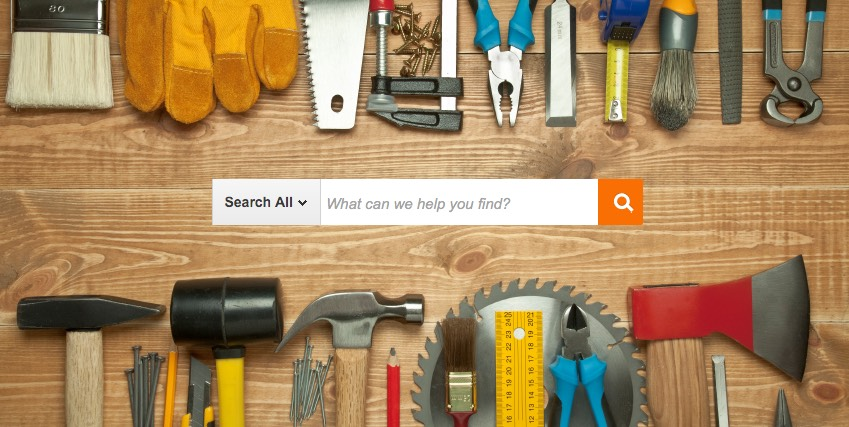
\includegraphics[width=0.5\textwidth]{home_depot_tools}
\caption{ Panorama built with three pictures}
\end{figure}
    
\end{block}
    %
    \begin{block}{IR algorithm: Lucene}
\small
We decided to use Apache Lucene because members of the team were used to it. It is a little bit more complicated version of tf-idf. It is used for instance by ElasticSearch.
\\ We run a script to build an index which lets to know the difference frequence of words in each file. It is then easy to know which products fits the best the query.

  \begin{figure}[H]
\center
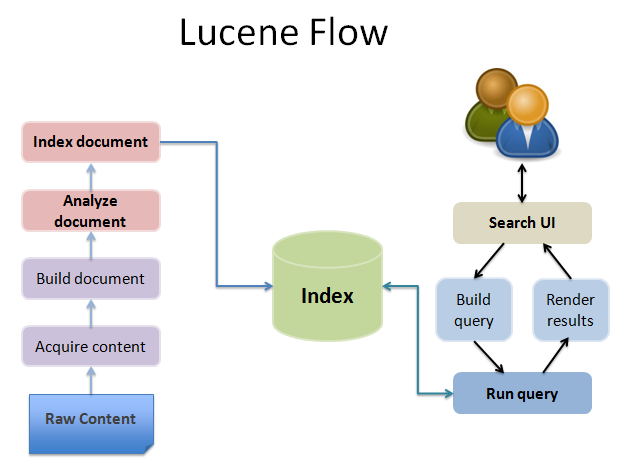
\includegraphics[width=0.5\textwidth]{lucence-flow}
\caption{ Panorama built with three pictures}
\end{figure}


    \end{block}
    %
\begin{block}{Results}
\small
      The competition leaderbord is based on a score computed on the Root mean Squared error compare to the score given human raters:
\begin{equation}
RMSE=\frac{1}{size(TestSet)} \sum_{(q_{i},p_{i})} (scorePredicted(q_{i},p_{i})-TrueHumanScore(q_{i},p_{i}))^{2}
\end{equation}
We are currently 885 over 1380 reaching a RMSE of 0.4913. The gap with 400th rank is only of 0.01.
    \end{block}
\end{column} 
    
  %
  \begin{column}[t]{\postercolumnwidth}
    \centering
\begin{block}{Datasets available}
\small
The task is thus to try to mimick the process made by a human rater to judge the quality of an output according to a particular query. For the task, we are provided several datasets: 
\begin{itemize}
\item the instructions given to a human rater 
\item some \textbf{descriptions of the different products} and some additional informations
\item\textbf{a training set} where we have access to the average grade given by a judge to a pair query-product returned by the algorithm
\item a test set where we need to \textbf{predict the relevance score for a particular pair query-product}
\end{itemize}
\textbf{Size of data sets}:
\begin{itemize}
\item product descriptions: we have 125000 product's description. 
\item training set: we have 74068 trio query-product-relevance score
\item test set: we need to predict the score of 16600 pairs of query-product
\end{itemize}     


    \end{block}
% 
 \begin{block}{Feature Engineering}
\small
We combined features based on Lucene together with traditional NLP features like words n-grams. Examples of our features are as follows:

\begin{itemize}

\item place of an answer in Lucene ranking crated for given query
\item Lucene score of an answer for given query
\item fraction of 1-grams/ 2-grams from query in answer's description/title/brand/attributes
\item average frequency of 1-grams/ 2-grams in answer's description/title 

\end{itemize}

\\
\textbf{Example:}
\\

    \end{block}
    % 
  \begin{block}{Ways of improvement}
\small
We understood that there was a lot of spelling mistakes in the descriptions and different ways to write different brand for example. By correcting those mistakes, the number of important words should increase: we belive that it could increase the performance of Lucene.
\\
\\
We implemented a grid search to find the best hyperameters of our models but it could be a good idea to implement a simple cross validation to compare the influence of the different features on our score.
\\
\\
Another way of improvement would be to try to combine our different machine learning algorithm to see if we can take advantage of their respective qualities.
    \end{block}
  \end{column}
  %
  \begin{column}[t]{\postercolumnwidth}
    \centering
     \begin{block}{Preprocessing}
 \small
The idea of our agorithm was to build our own search engine and then try to see the results of the query. we then check the rank of the product we want to match in the query result to build a feature. We try to build different scores and then try to unify them through the training of a regressor on the training set provided by Home Depot. 
\\Preprocessing steps to build our IR algorithm (use of several python libraries): 
\begin{itemize}
\item nltk word tokenization: just tokenize the data
\item stopwords removal: delete all the useless words in the description of the product
\item porter stemming: our IR algorithm will be based of frequences of words: thus stemming lets to avoid having lot of different words of the same family with small frequences
  \begin{figure}[H]
\center
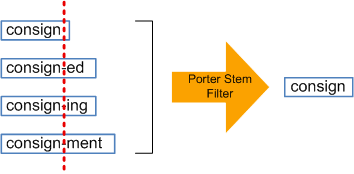
\includegraphics[width=0.5\textwidth]{figure3}
\caption{ Panorama built with three pictures}
\end{figure}
\item create a text fil for each product
\end{itemize}
   \begin{figure}[H]
\center
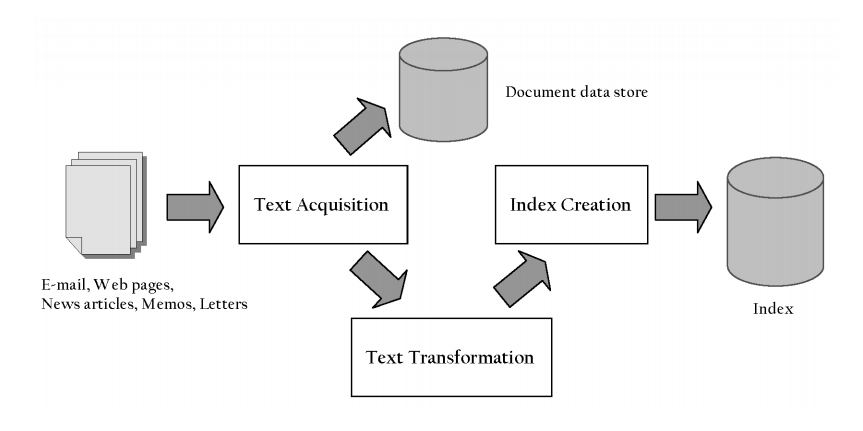
\includegraphics[width=0.5\textwidth]{index}
\caption{ Panorama built with three pictures}
\end{figure}
    \end{block}


    \begin{block}{Machine Learning algorithm}
\small
To try to train build our predicter on the different features we build we tried to train several algorithms. In all cases, we used the algorithms pre-implemented in scikitlearn.  
\begin{itemize}
\item Single Vector Machine regressor
\item Random Forest 
\item Adaboost regressor
In all cases, we implemented grid search to try to find best parameters
\\
Random forest is very fast to train and is is the algorithm which has given us the best score so far. 
\end{itemize}


    \end{block} 

    \begin{block}{Conclusion}
\small
This challenge is very interesting because the task is not only to find a very good search engine but to try to mimik the process of a human to determine if a document is relevant or not for a particular query. 
\\ We hope to increase our score in the Kaggle leaderbord. However, because the scoresare very tight between the 400th and 800th we think we are on the right path.
    \end{block}
  \end{column}
 \end{columns}

\end{frame}



\end{document}
